\documentclass[twoside,10pt,a4paper]{article}
\usepackage{graphicx}
\graphicspath{ {./images/} }
\usepackage[english]{babel}					
\usepackage[T1]{fontenc} 					
\usepackage[utf8]{inputenc}						
\usepackage{helvet}					
\renewcommand{\familydefault}{\sfdefault}
\usepackage{microtype}						
\usepackage{blindtext}
\usepackage{csquotes}
\usepackage[onehalfspacing]{setspace}			
\usepackage{geometry}				               
\geometry{left=4cm,right=4cm,top=3cm,bottom=6cm}
\pagestyle{plain}						            
\usepackage{mathtools} 							
\numberwithin{equation}{section}			
\numberwithin{figure}{section}						
\usepackage[version=4]{mhchem}						
\usepackage{siunitx}								
\sisetup{detect-all, detect-weight=true, detect-family=true}  
\sisetup{range-units=single}  						
\sisetup{multi-part-units=single}				
\sisetup{separate-uncertainty}				
\usepackage{caption}
\usepackage{graphicx}								
\usepackage[section]{placeins}				
\usepackage{array} 							
\usepackage{booktabs}							
\usepackage[backend=biber,citestyle=numeric-comp,bibstyle=numeric,sorting=none,url=false,eprint=false,isbn=true,doi=true]{biblatex}
\addbibresource{./example.bib}	
\usepackage{hyperref, bookmark}					
\hypersetup{colorlinks=true,linkcolor=black,citecolor=blue,urlcolor=blue}
\begin{document}
\fontfamily{phv}\selectfont
\begin{titlepage}			
	\centering
	{\scshape\LARGE Indian Institute of Technology Kanpur\par}
	\vspace{1cm}
	{\huge\bfseries CS253-Assignment 5\par}
	\vspace{1cm}
	{\Large\itshape Soham Ghosal\par}	
	\vspace{1cm}
	\begin{center}
	    Roll:180771
	\end{center}
	\vspace{1cm}
	{\large \today\par}
	\vspace{3cm}
	\includegraphics[scale=0.25]{Rohit.jpg}
\end{titlepage}
\section{Introduction}\label{sec:section1}			
\textbf{Rohit Gurunath Sharma} (born 30 April 1987) is an \textbf{Indian international cricketer} who plays for Mumbai in domestic cricket and captains Mumbai Indians in the Indian Premier League as a right-handed batsman and an occasional right-arm off break bowler. He is the \textbf{vice-captain} of the Indian national team in limited-overs formats. \textbf{Under his captaincy, India won the Asia Cup and Nidahas Trophy in 2018.} \par
Outside cricket, Sharma is an active supporter of \textbf{animal welfare campaigns}. He is the \textbf{official Rhino Ambassador for WWF-India} and is a member of People for the Ethical Treatment of Animals (PETA). He has worked with PETA in its campaign to raise awareness of the plight of homeless cats and dogs in India.
\section{Career Statistics}
Below, I have tried to summarise the major statistics in his career.
\subsection{Number of Matches played in each format}
As of $24^{th}$ March,2021, Rohit Sharma has played 1111 matches across all formats.The number of matches per format is shown below.Since the data is categorical, a pie chart is a very good way to represent it.Rohit has played 38 Tests, 225 ODIs, 111 T20Is, 98 First Class Matches, 296 List A Matches and 343 T20s
\begin{flushleft}
    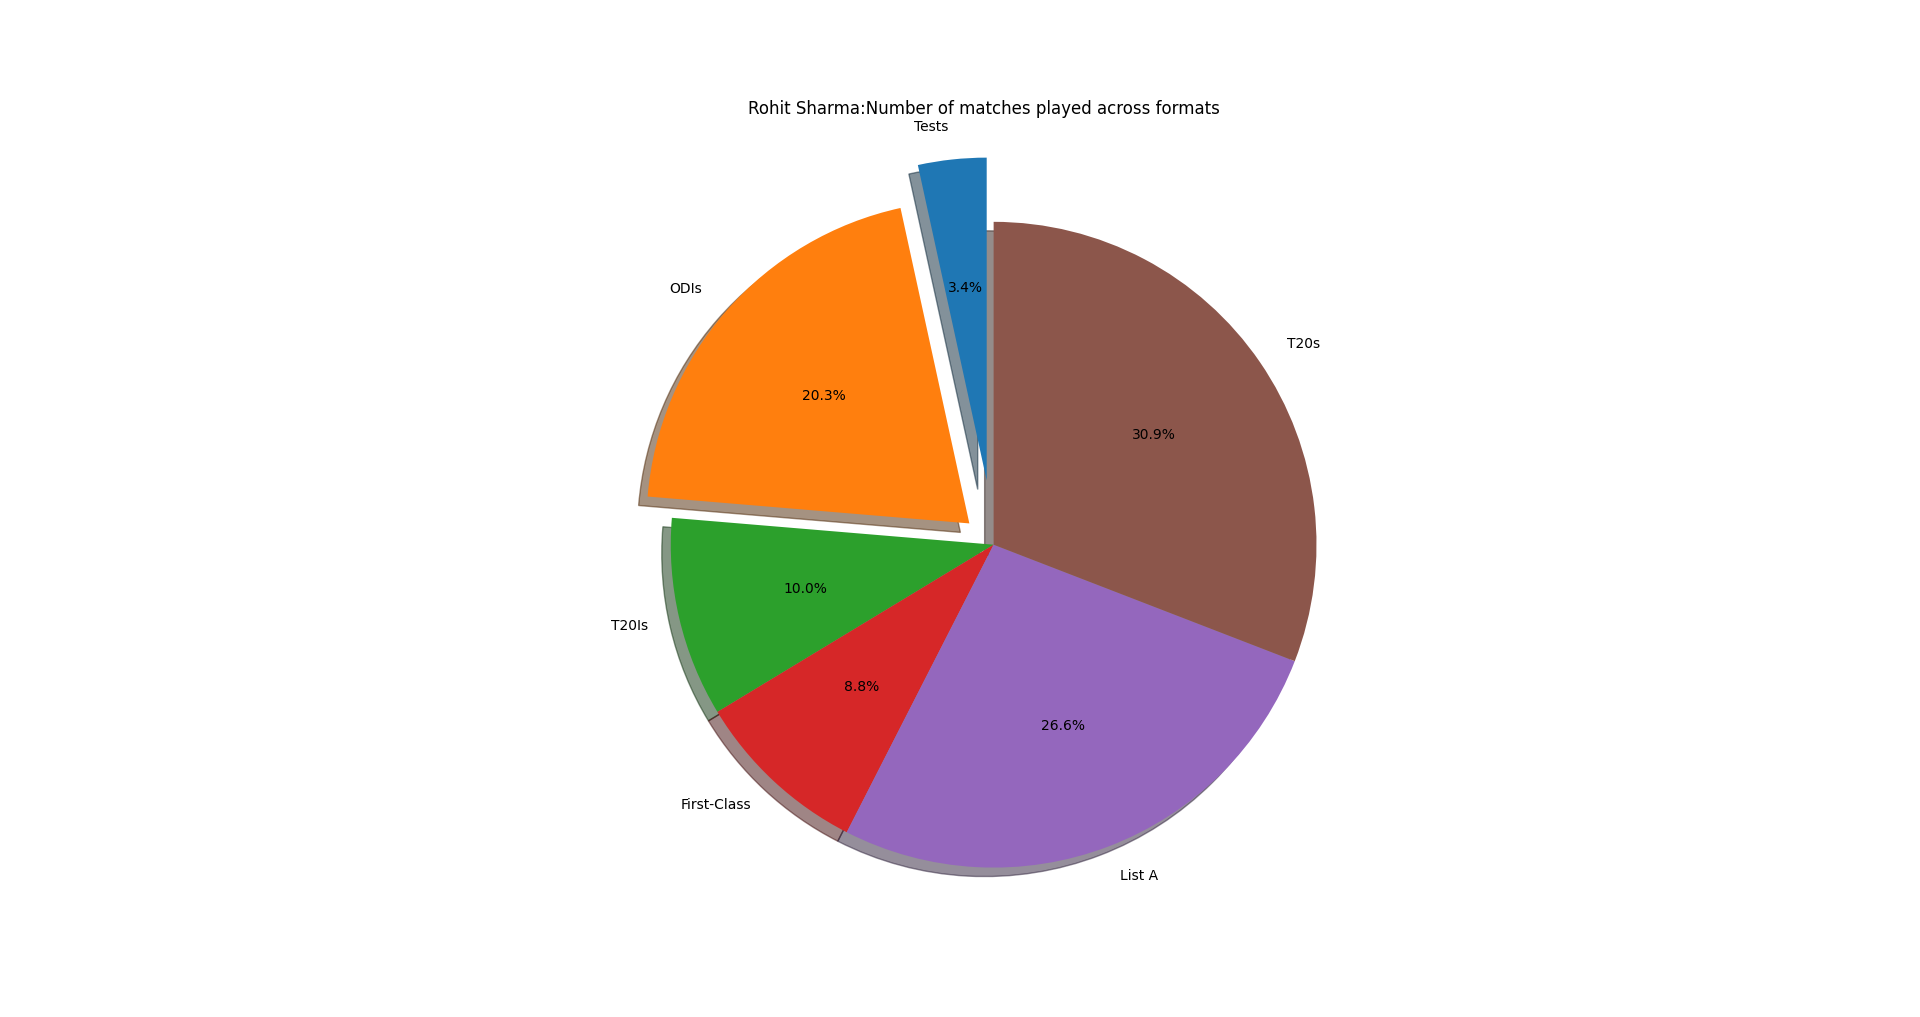
\includegraphics[scale=0.30]{matches.png}
\end{flushleft}
\subsection{Batting Average across all formats}
In cricket, batting average is defined as the total number of runs scored by a player divided by the number of times the player got out.Usually in the longer format of the game, an average of 40+ is considered very good, whereas in T20Is, an average of 30+ would be considered excellent. If we look at the bar graph for Rohit, he has an average of over 40 in every longer format of the game, whereas in T20s his average crosses 30. This is a hallmark of his consistency throughout all formats.
    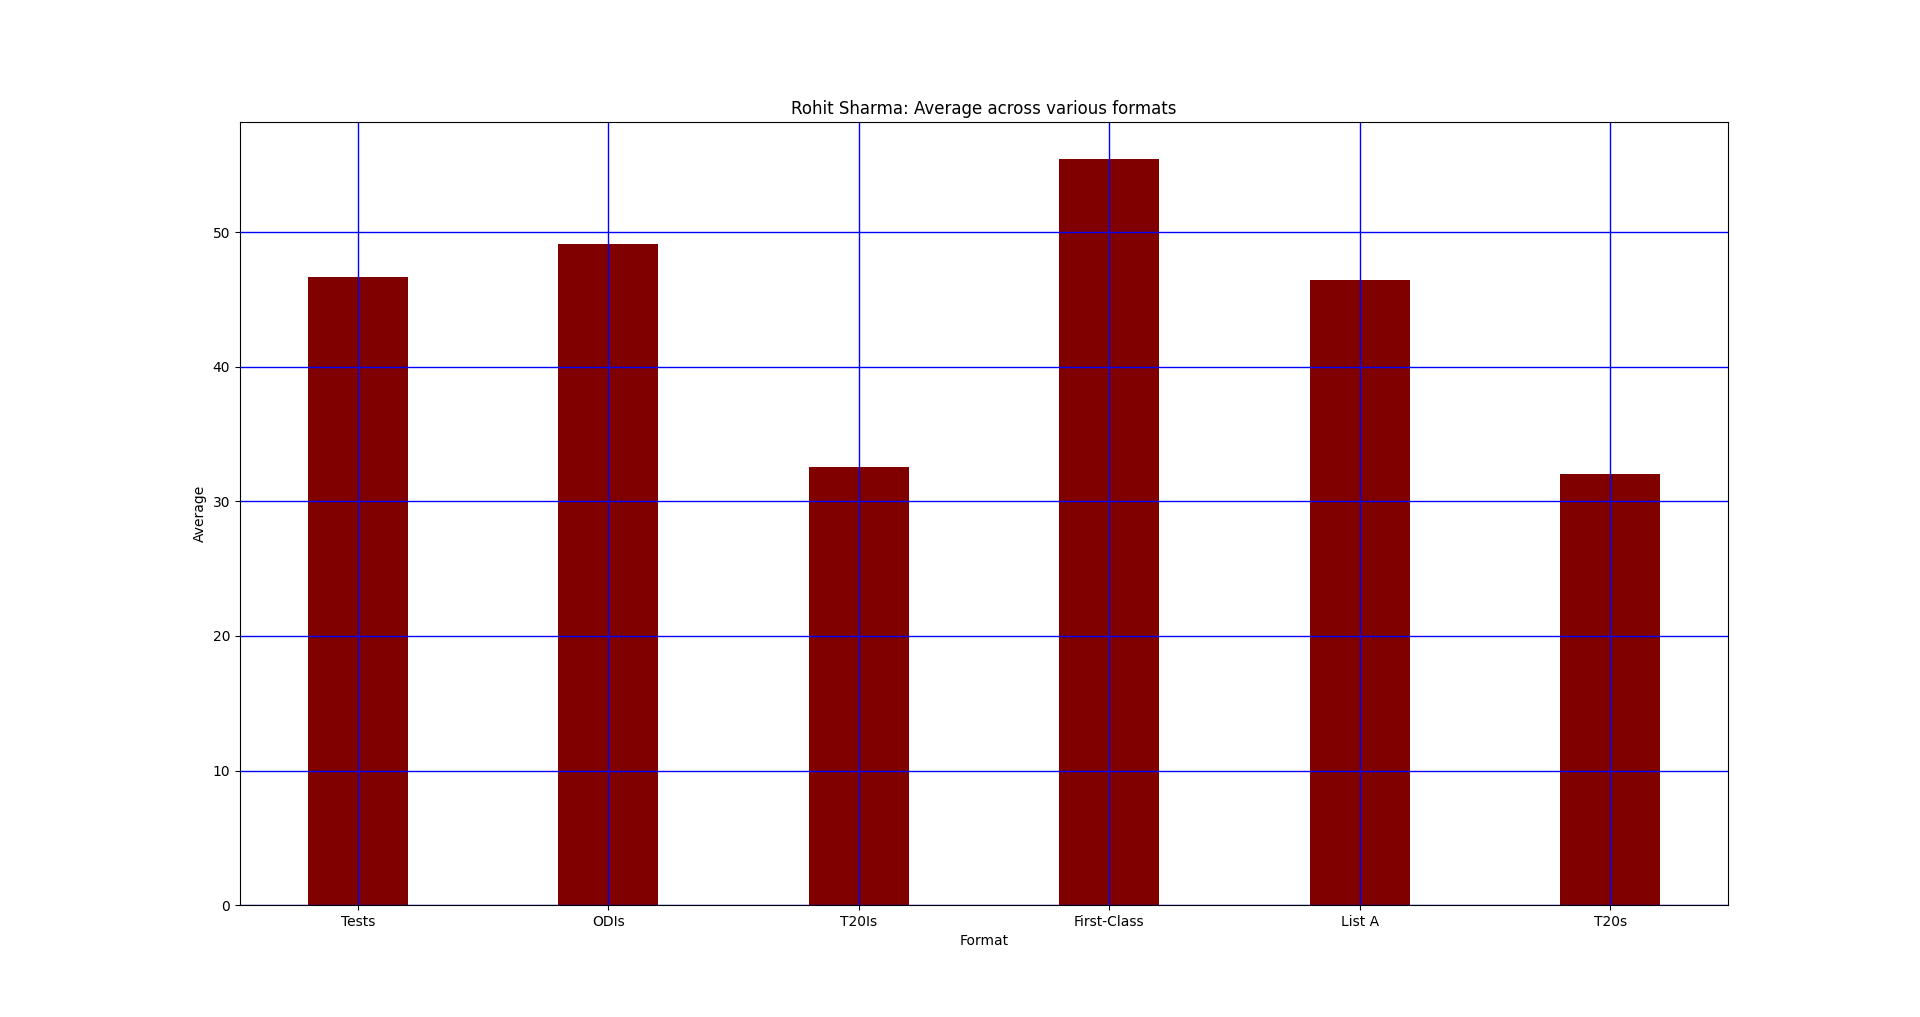
\includegraphics[scale=0.23]{Average.png}
\subsection{Batting Strike Rate across all formats}
In today's modern cricketing era, runs are not the only parameter to gauge someone's excellence. In this modern era where every batsman is equipped with a plethora of shots all around the wicket, it is very important for any batsman to accelerate whenever required and play with a good strike rate. Strike rate is defined as the average runs scored per 100 balls faced. Usually, S/R of more than 100 is considered good in ODIs and T20Is.
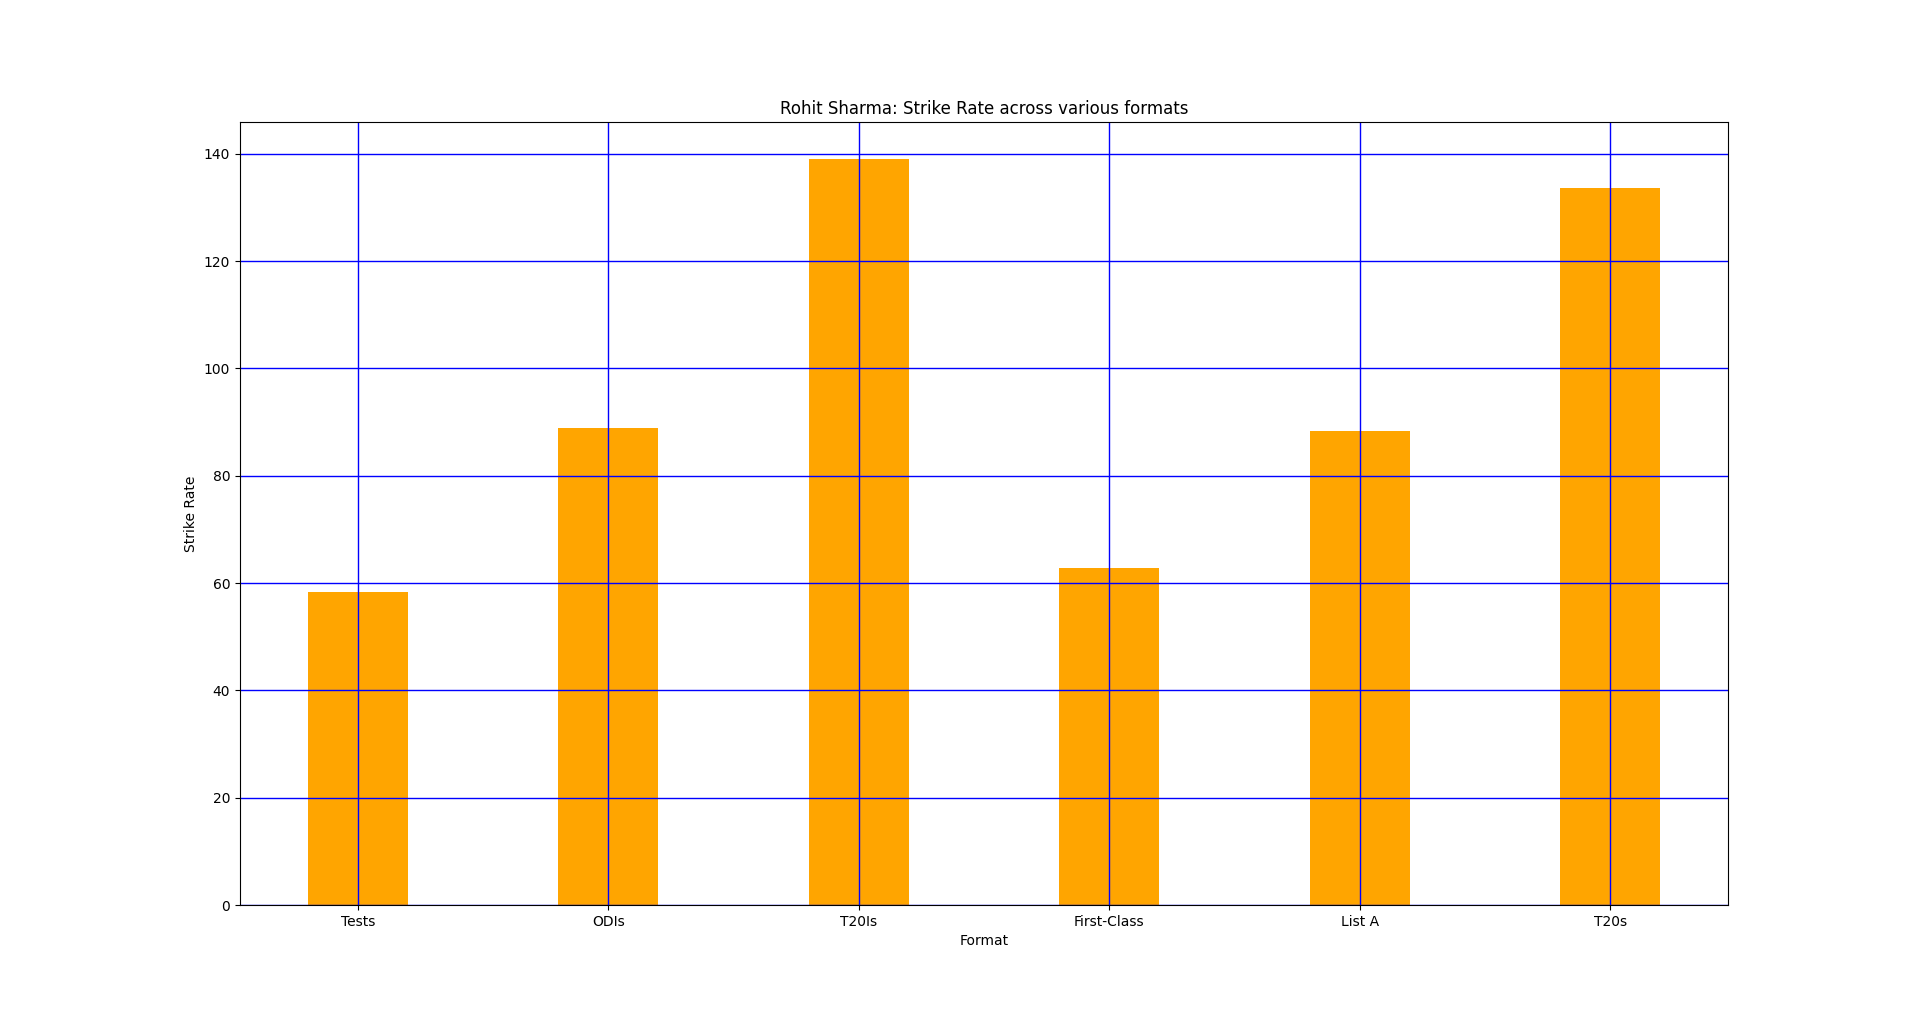
\includegraphics[scale=0.23]{Strike_rate.png}
\subsection{Position-wise batting Average}
In the initial phases of his career, Rohit played as a middle order batsman, coming in at 6 or 7.He did score some important runs coming in late, but never got to utilise his full potential, mainly because by the time he came in, only a few balls would be left. His fortunes took a turn in 2013, when he was promoted to open for India in the Champions Trophy. He scored a lot of runs in the opening position.While opening, both his Test and ODI average is almost 60, which is insane.
\begin{center}
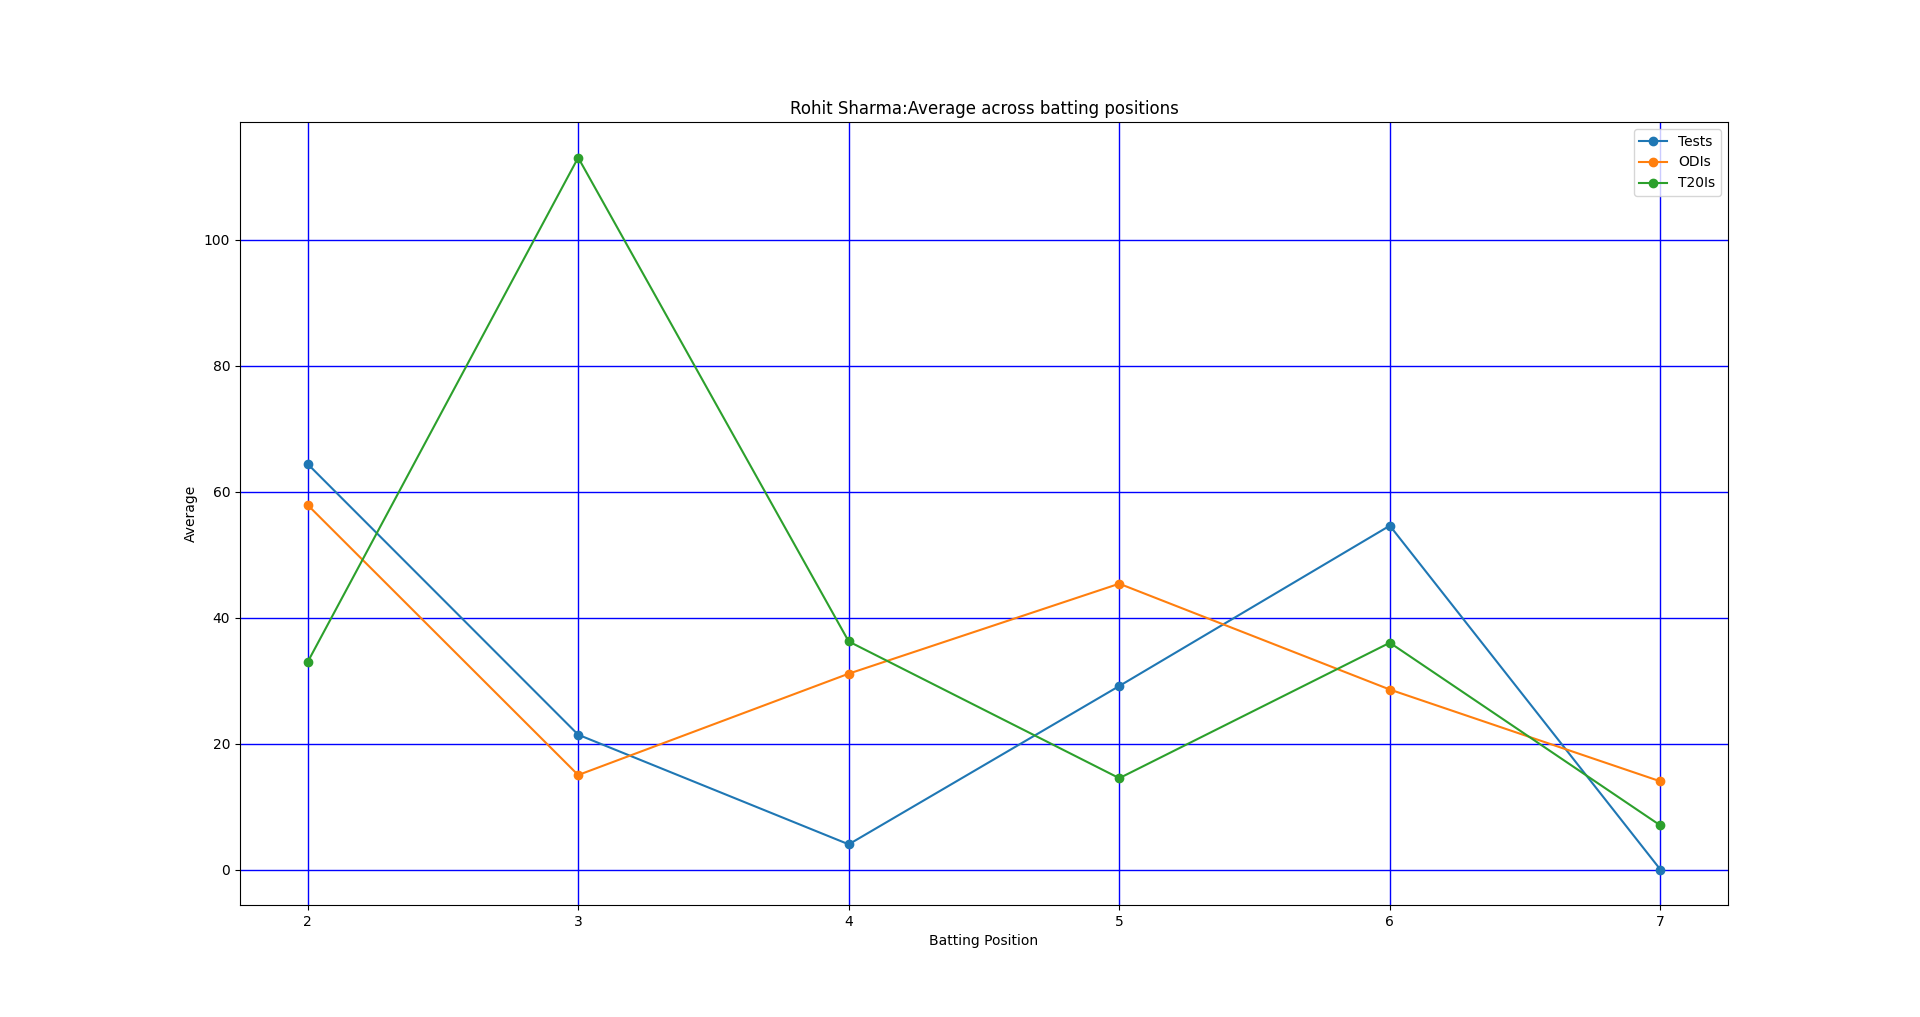
\includegraphics[scale=0.24]{avg_battingpos.png}    
\end{center}
\subsection{Centuries and Half Centuries across all formats}
This grouped bar plot shows the count of his centuries and half centuries across all formats.Note that he has 7 centuries and 12 half centuries at the Test level, and 29 centuries and 43 half centuries in ODIs. Such a conversion rate is very rare in modern day cricket, and this is one of the reasons why he is rated highly as a batsman.
\begin{center}
    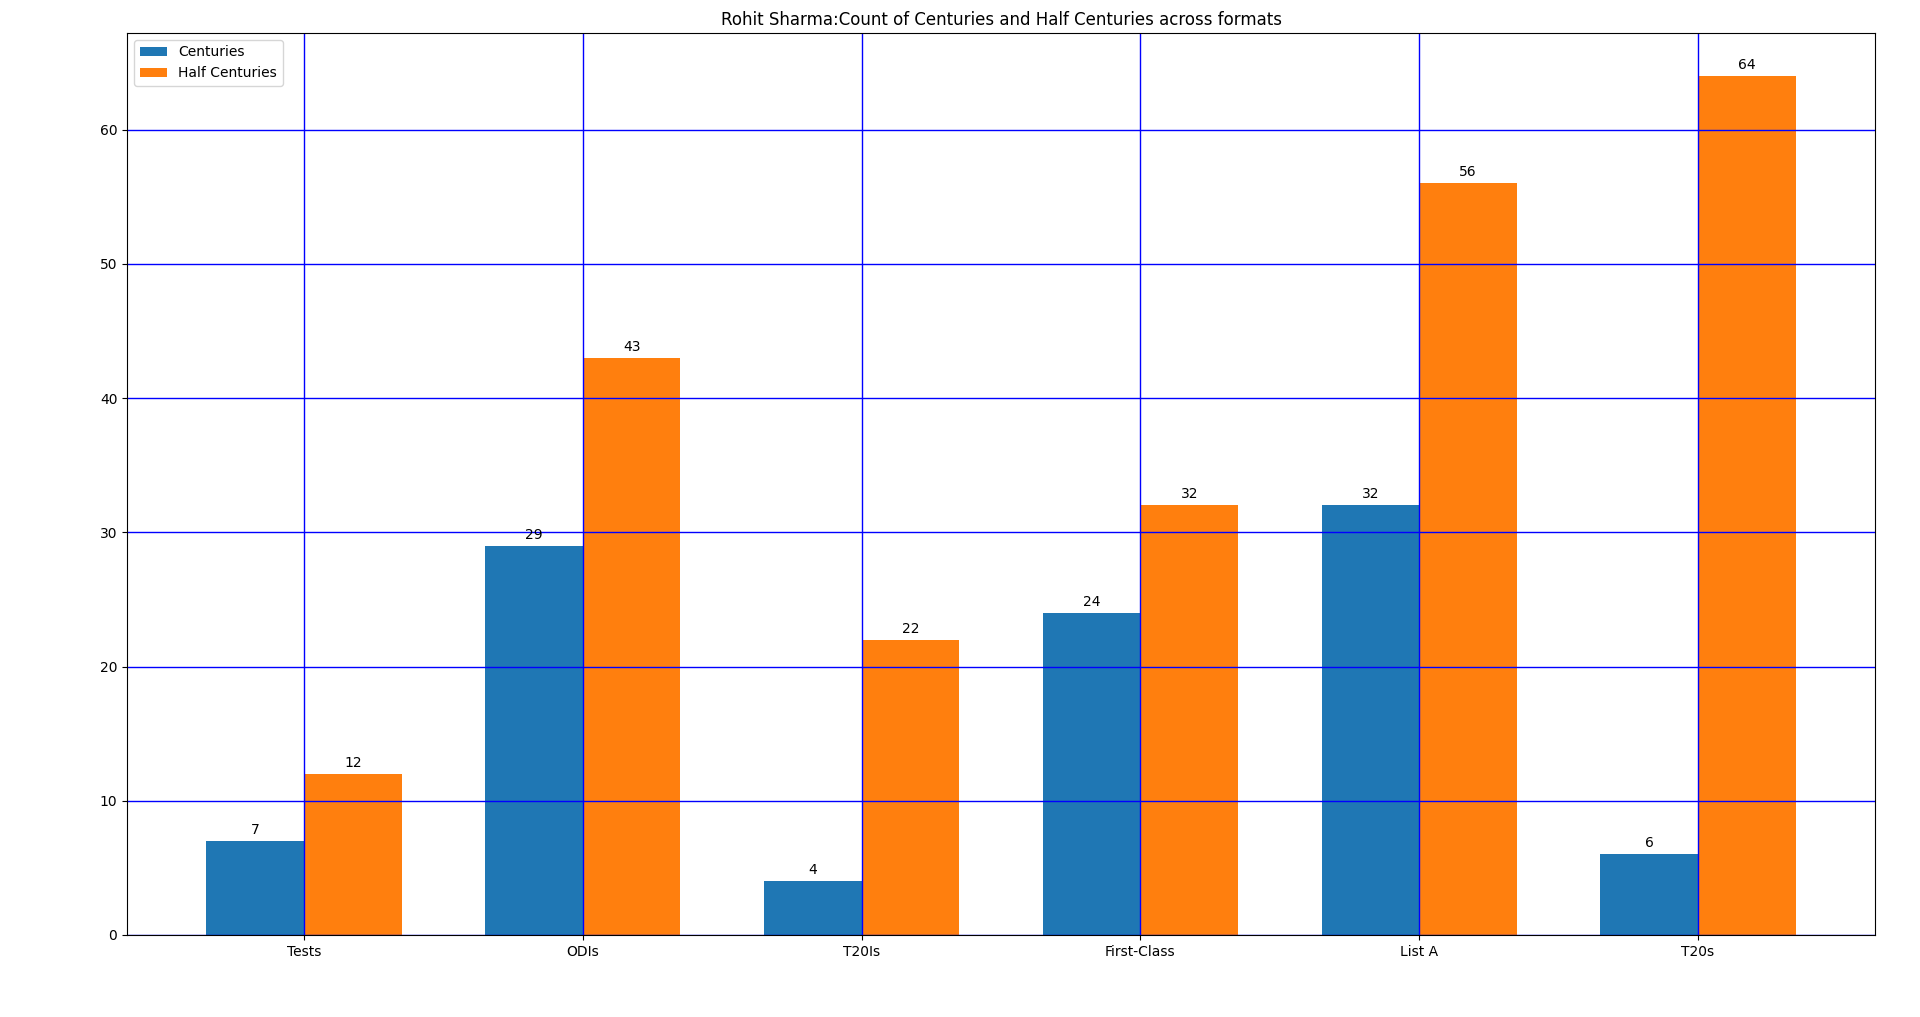
\includegraphics[scale=0.25]{100s50s.png}
\end{center}
\subsection{Runs scored against each opponent}
The next grouped bar plot shows the runs scored against every opponent in Tests, T20Is and ODIs.The tall blocks corresponding to ODIs, really show how dangerous a player he is at the top of the innings.Also, he has scored the most runs in ODIs against Australia,Sri Lanka and West Indies
\begin{center}
    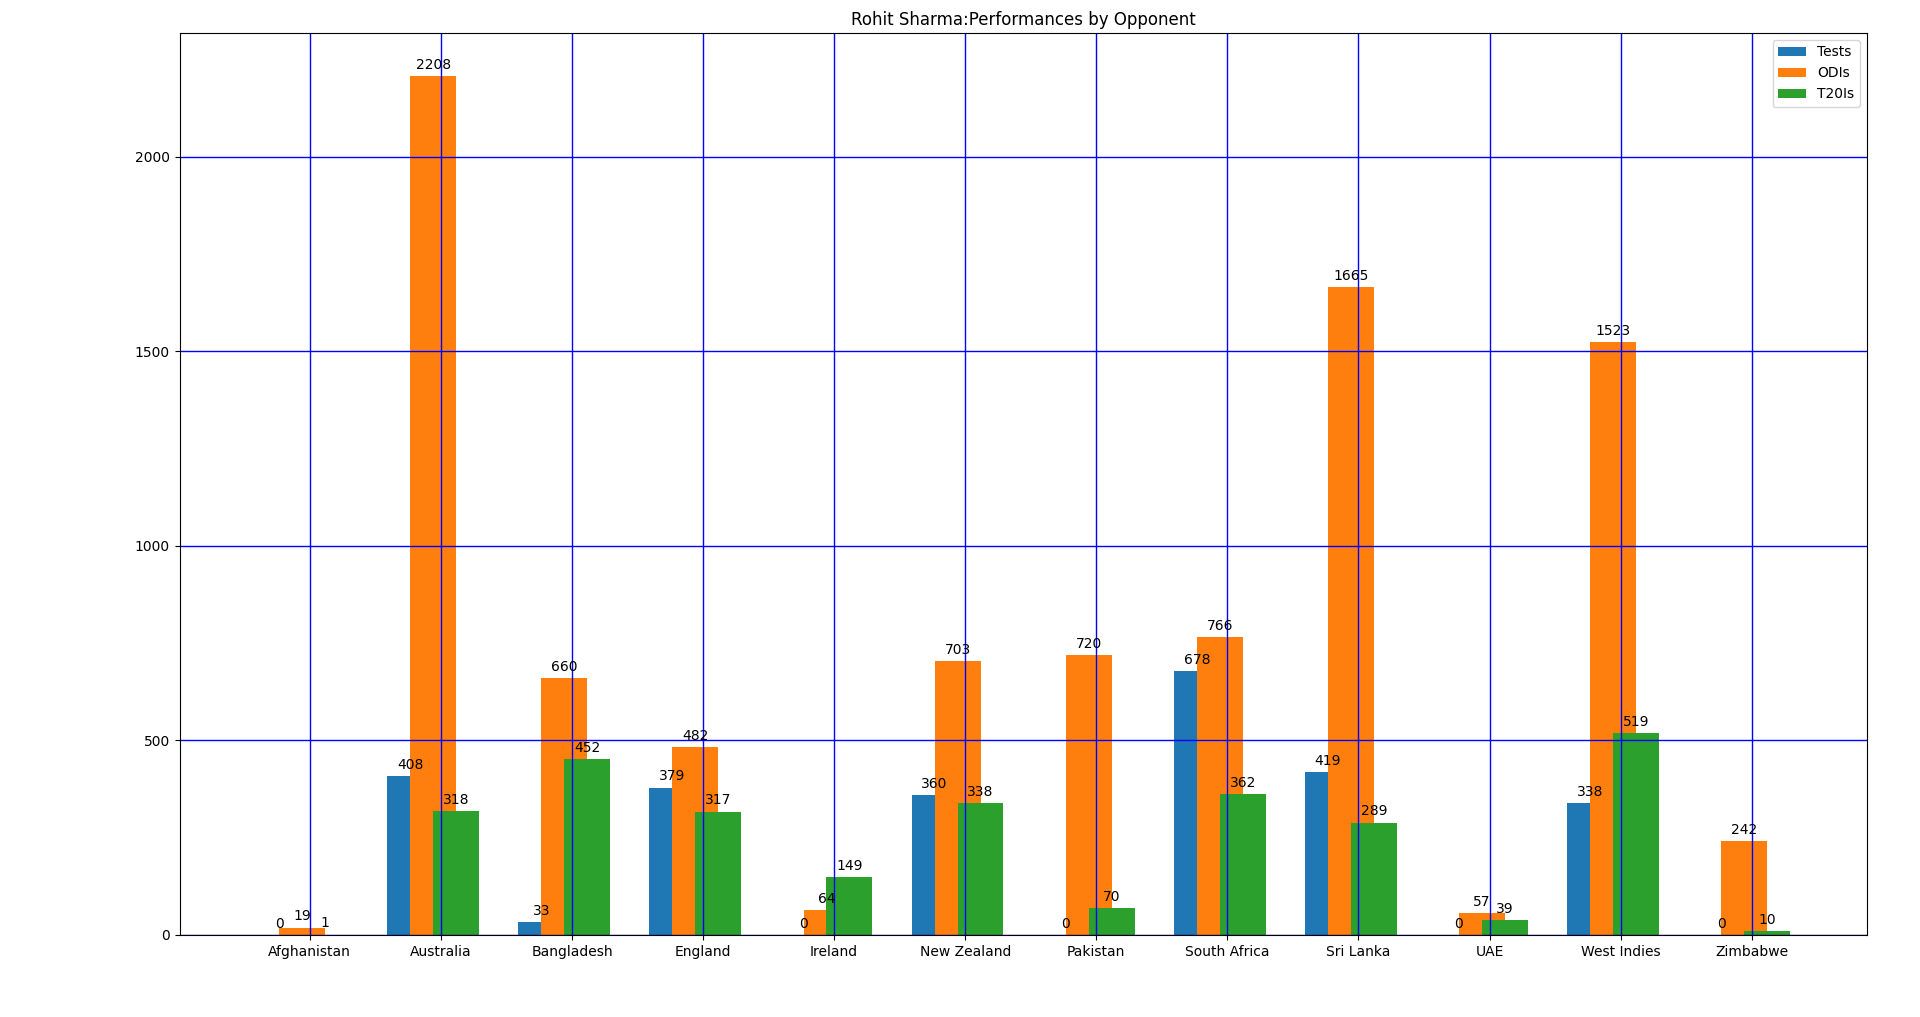
\includegraphics[scale=0.23]{Performance_opponent.png}
\end{center}
\subsection{Runs scored across different venues}
The next graph is a grouped bar chart, which shows how many runs he has scored in each country. This graph gives us a lot of information about his technique and pitch preferences. We see that in terms of total runs, he has scored the most in India, where the pitches are kind of sluggish.A significant chunk of his ODI runs have come in Australia and England, where the pitches are grassy, full of pace and bounce.Also, small blocks corresponding to the test field, shows that he is pretty vulnerable to swing outside the subcontinent.
\begin{center}
    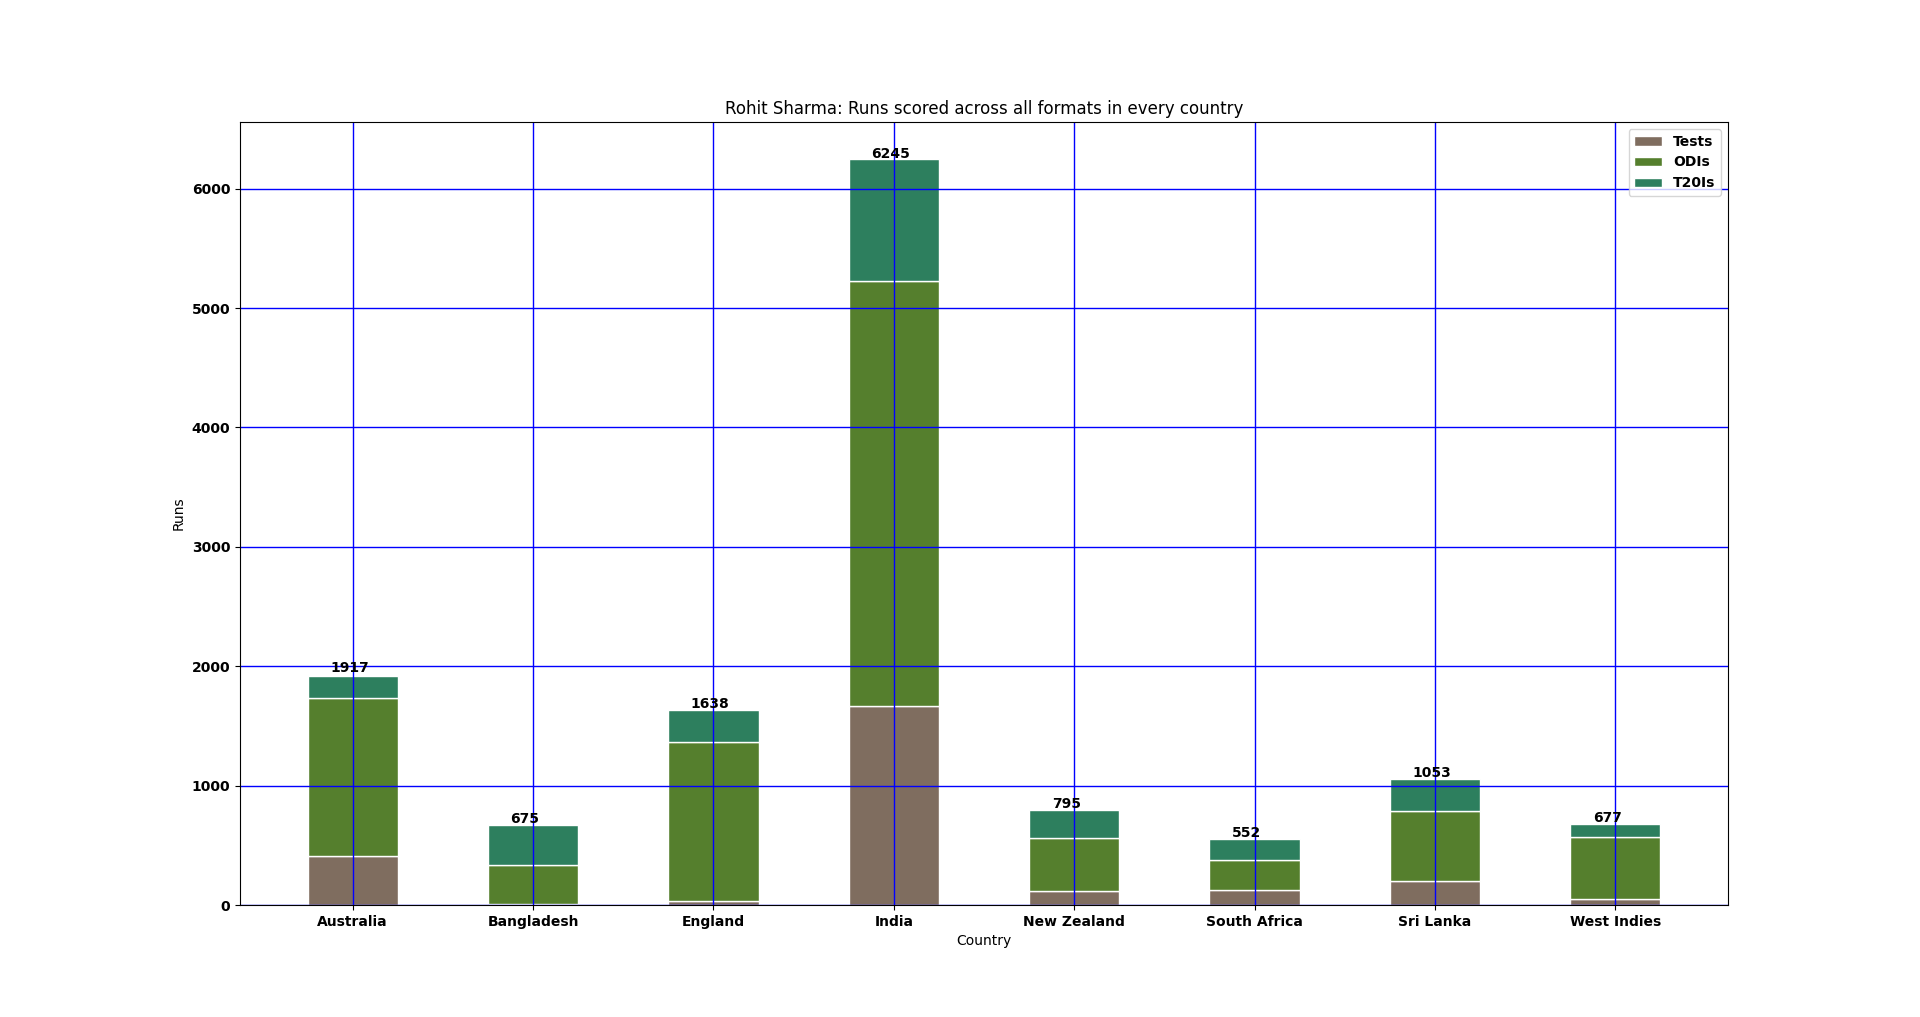
\includegraphics[scale=0.24]{runspercountry.png}
\end{center}
\subsection{Total runs in every calendar year}
This is a line graph which shows how many runs he has scored in every format throughout the years.The overall graph is kind of monotonic, but there is a significant leap after 2013, thanks to his promotion to the opening slot in 2013 champions trophy.Also, we note that the ODI graph is miles ahead of both his T20 and Test runs, which explains why he is regarded as such a dangerous ODI batsman.
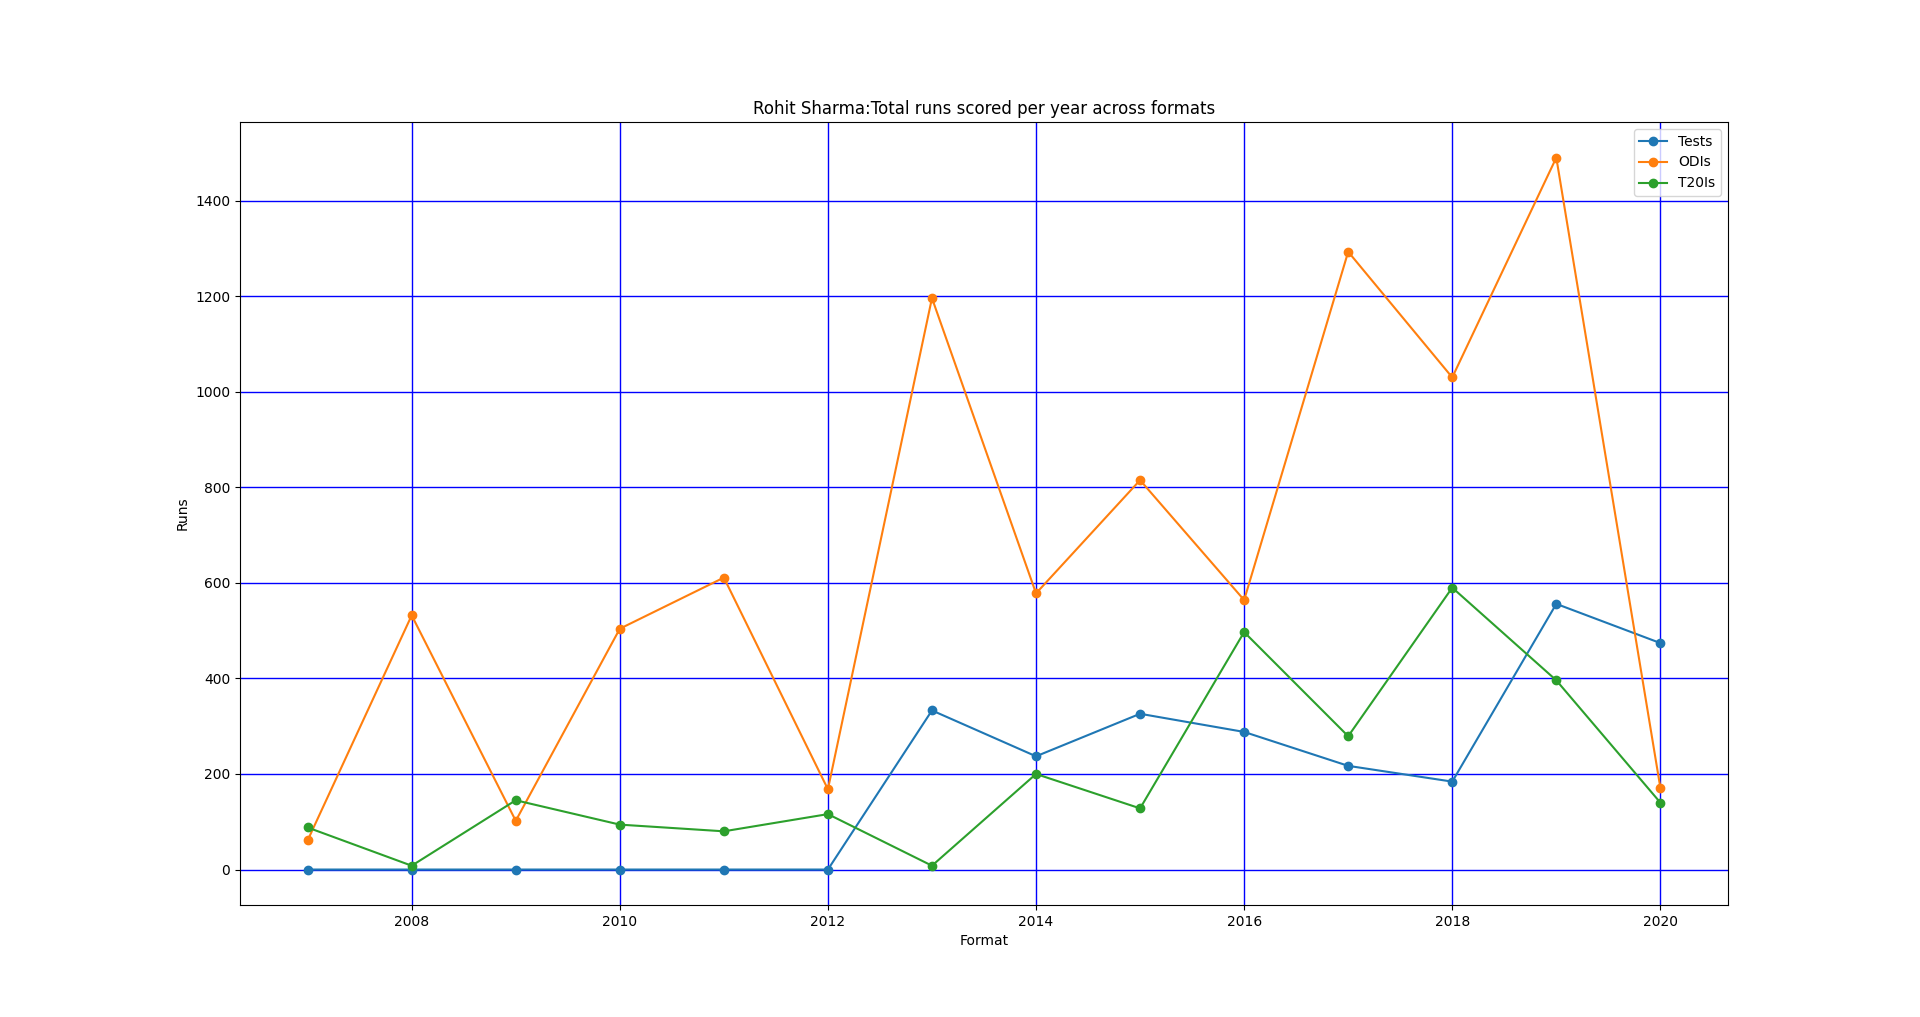
\includegraphics[scale=0.24]{Totalruns.png}
\subsection{Mode of Dismissals}
\subsubsection{Tests}
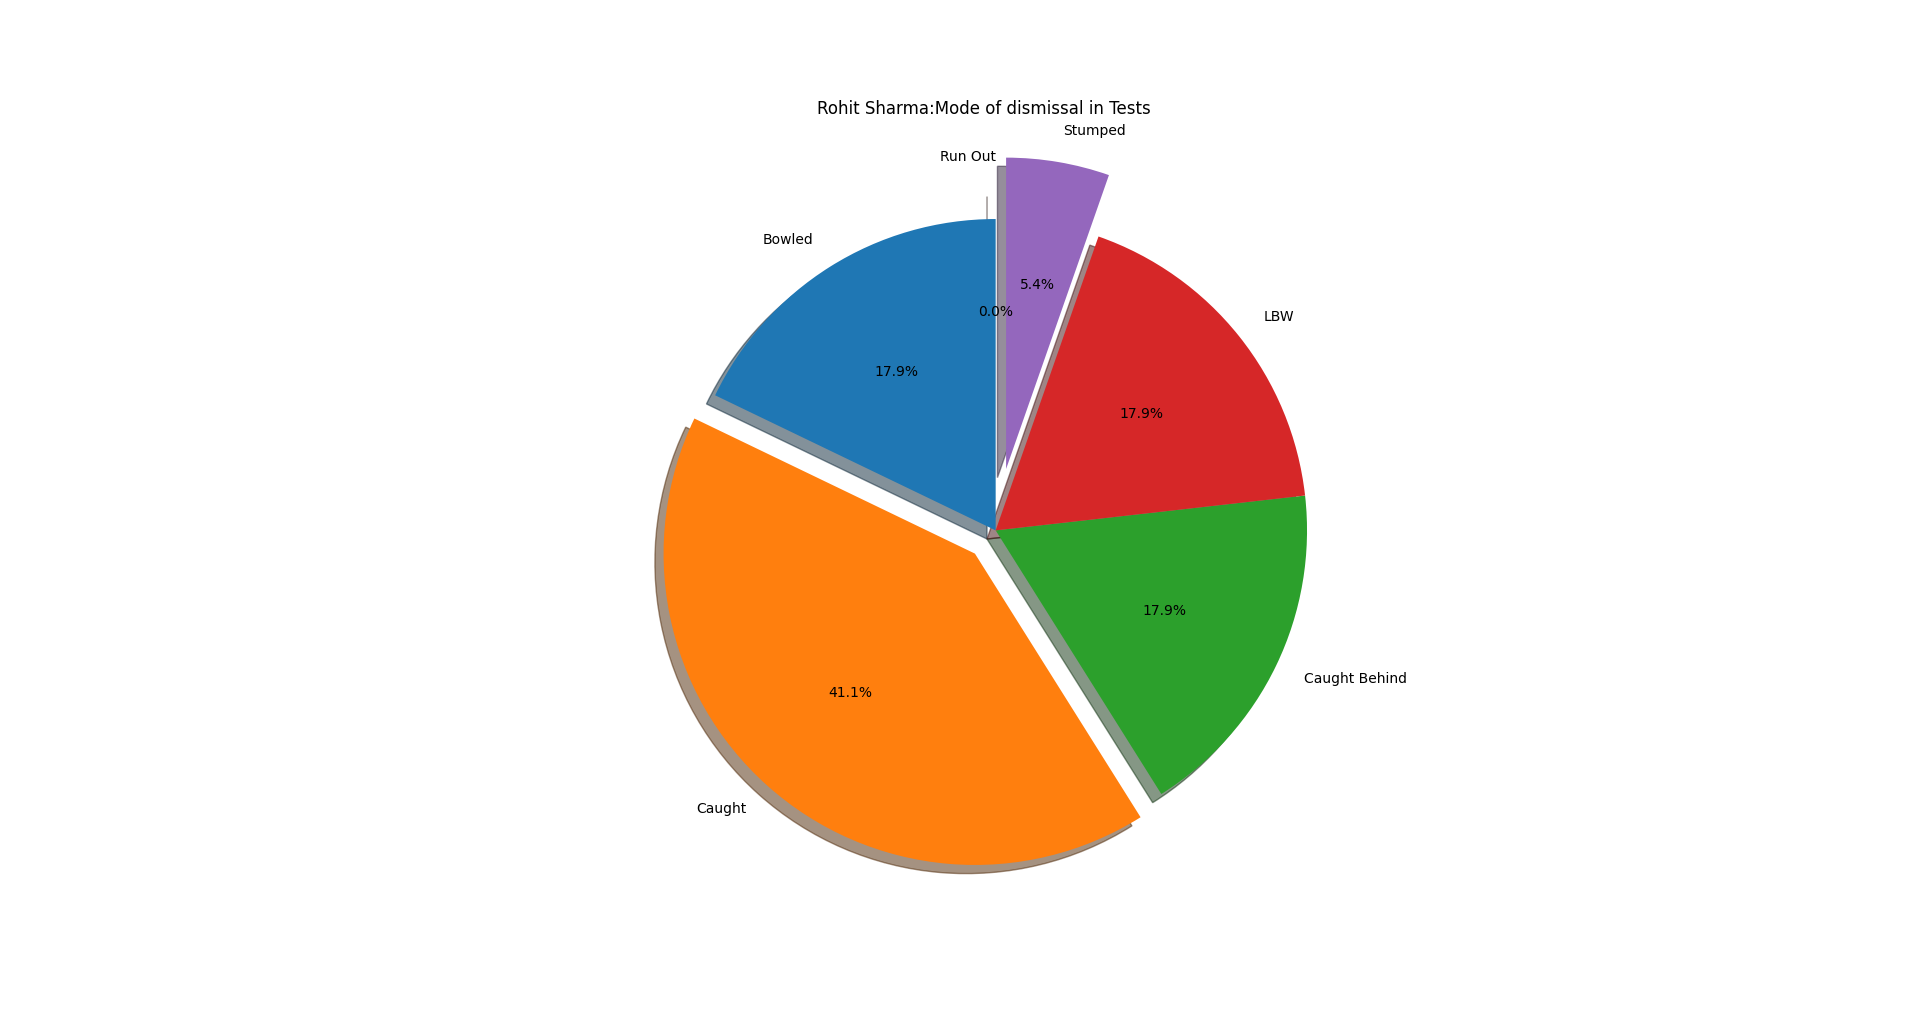
\includegraphics[scale=0.30]{Modeofdismissal_Tests.png}
\subsubsection{ODIs}
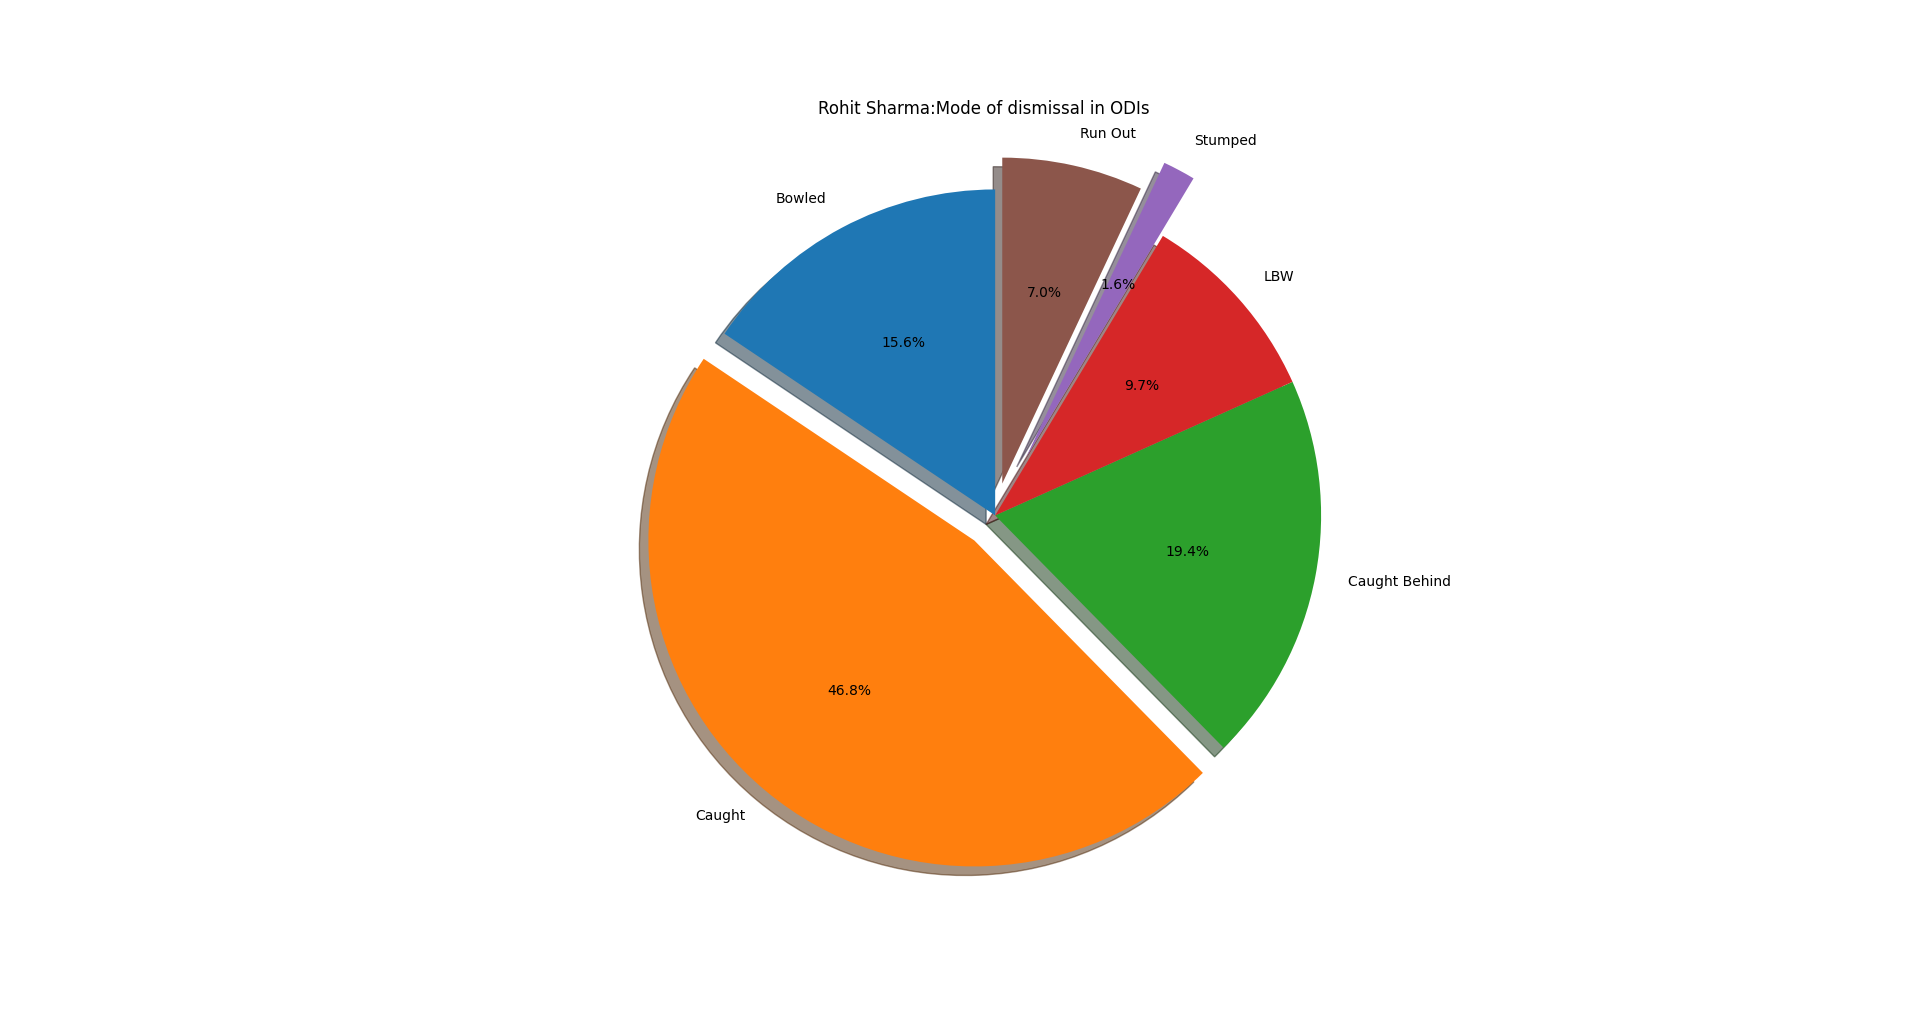
\includegraphics[scale=0.30]{Modeofdismissal_ODI.png}
\subsubsection{T20Is}
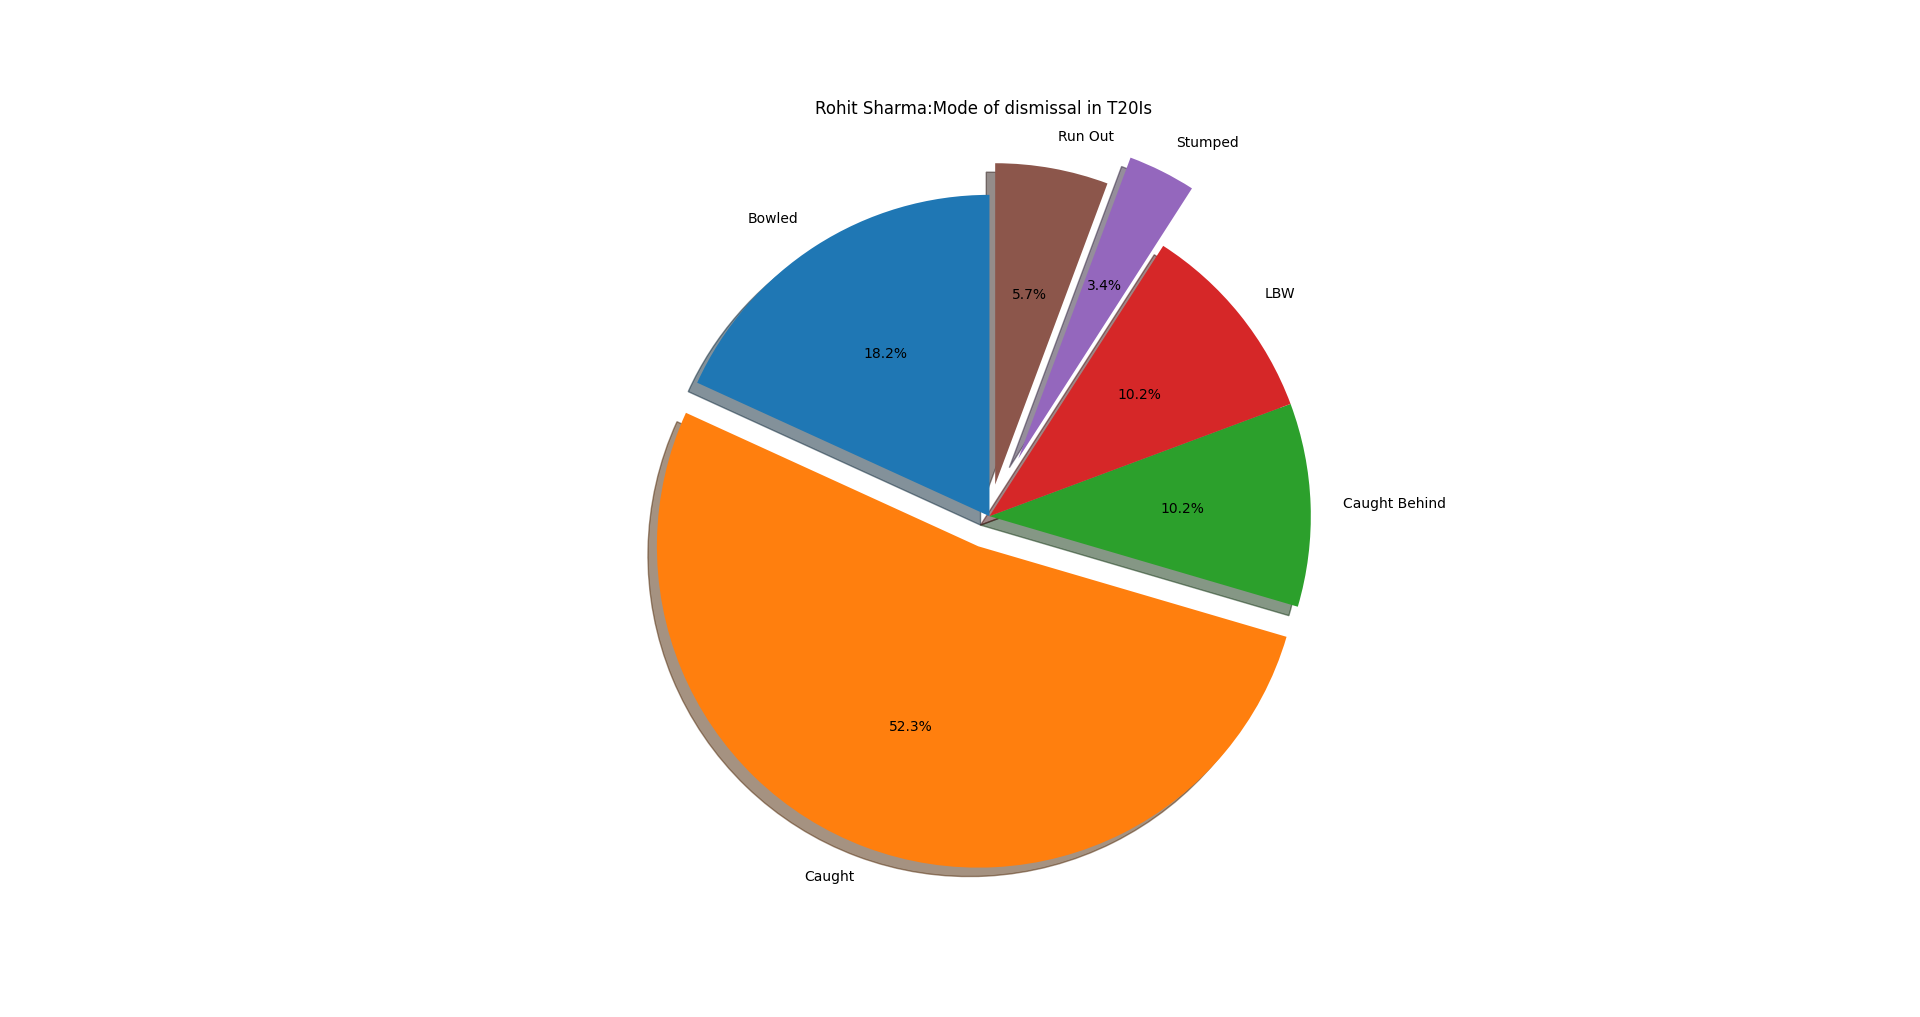
\includegraphics[scale=0.30]{Modeofdismissal_T20Is.png}
What we can conclude from these 3 pie charts is: A significant number of dismissals is due to LBW. If we analyze some of Rohit's dismissals, it will be clear that he is vulnerable to the moving ball in the initial phase of his stay at the crease. If he can work on this aspect of the game, he would perform much better, both in Tests, and in ODIs and T20Is outside the subcontinent, where the ball seams and swings lot more.
\subsection{Home vs Away--Comparison}
A cricketer spends the majority of his career playing in his home country. Thus it is expected that his stats will be the best in his home country. The greatness of a batsman is often gauged by how he plays outside his home, specially in different conditions. For example, an Indian batsman would be gauged by his performances in England or AUstralia, where the pitch is fast and bouncy. In contrast, an Australian Batsman, would be expected to do well in the Indian Subcontinent, where the pitch is slow and sluggish with uneven bounce.
Thus, Home Vs Away is an important comparison in cricket. Below, I have plotted two group bar charts--the first one showing Rohit's runs in home conditions and away conditions, while the second one shows the total number of centuries across all formats.
\subsubsection{Total runs}
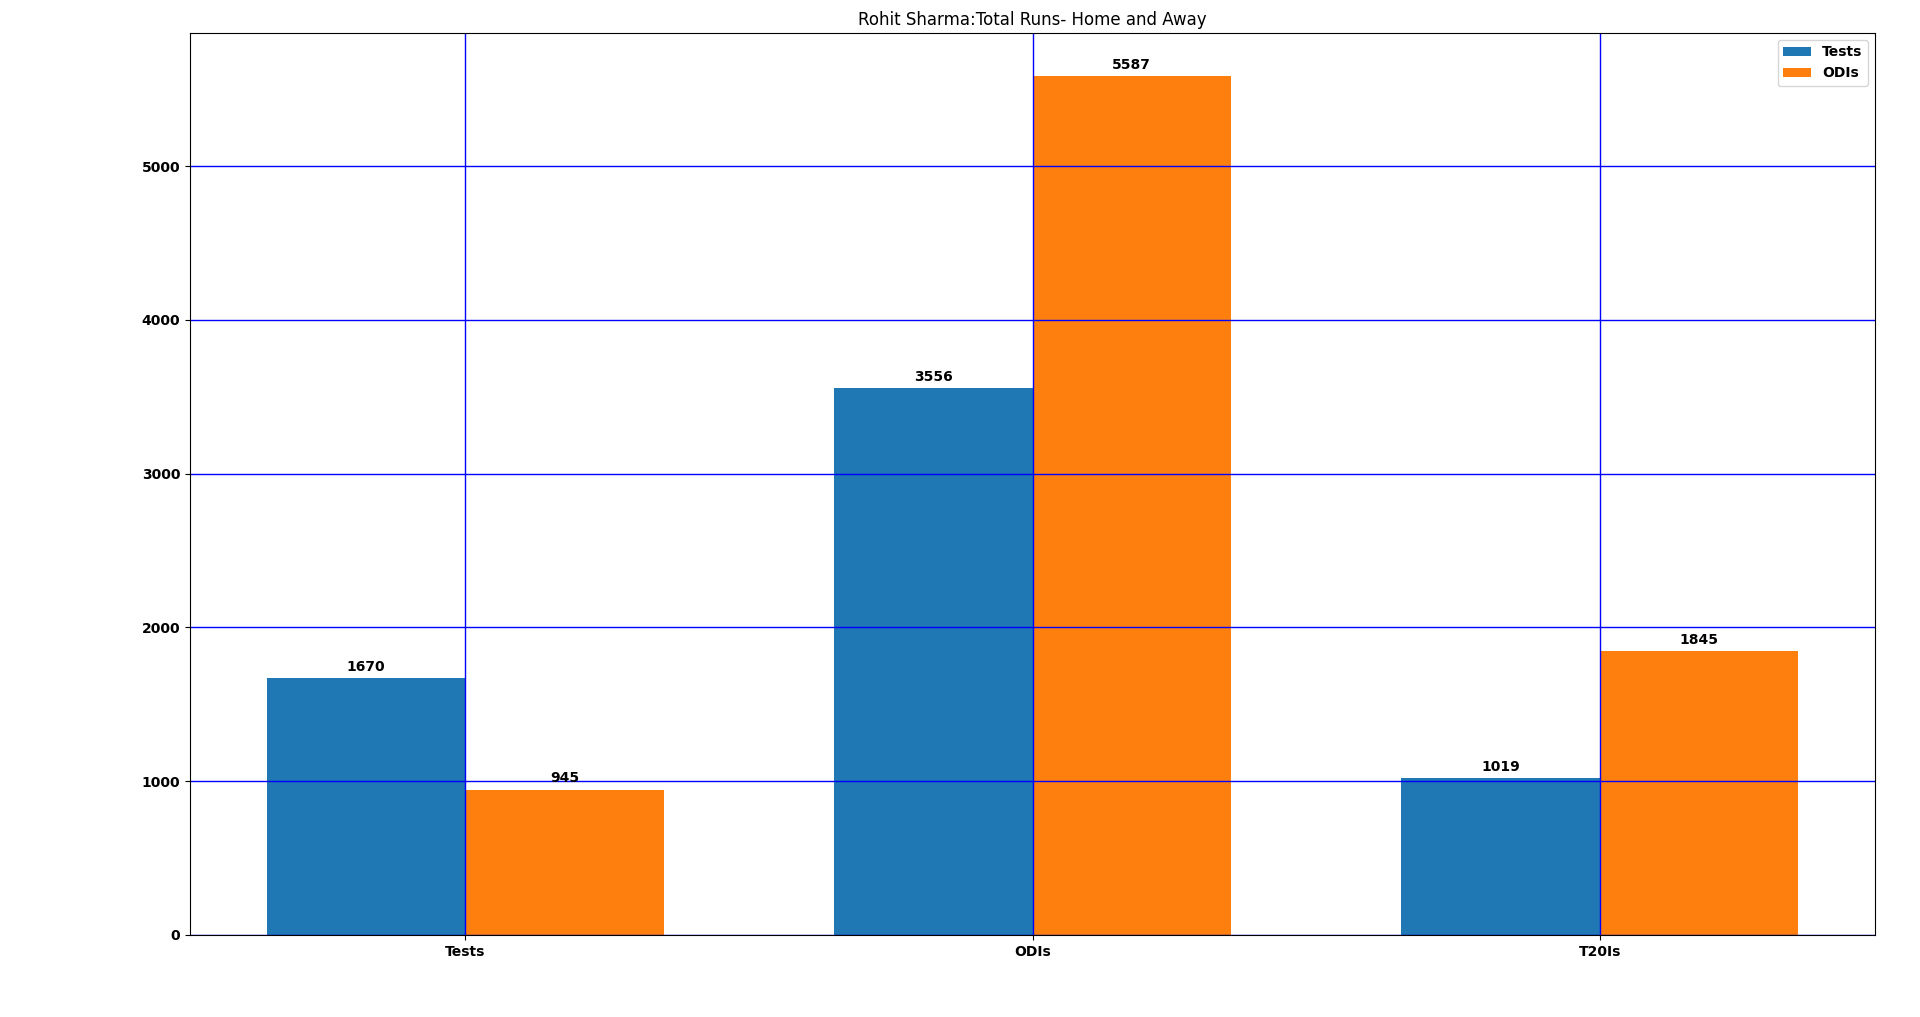
\includegraphics[scale=0.22]{Home_away_runs.png}
\subsubsection{Centuries}
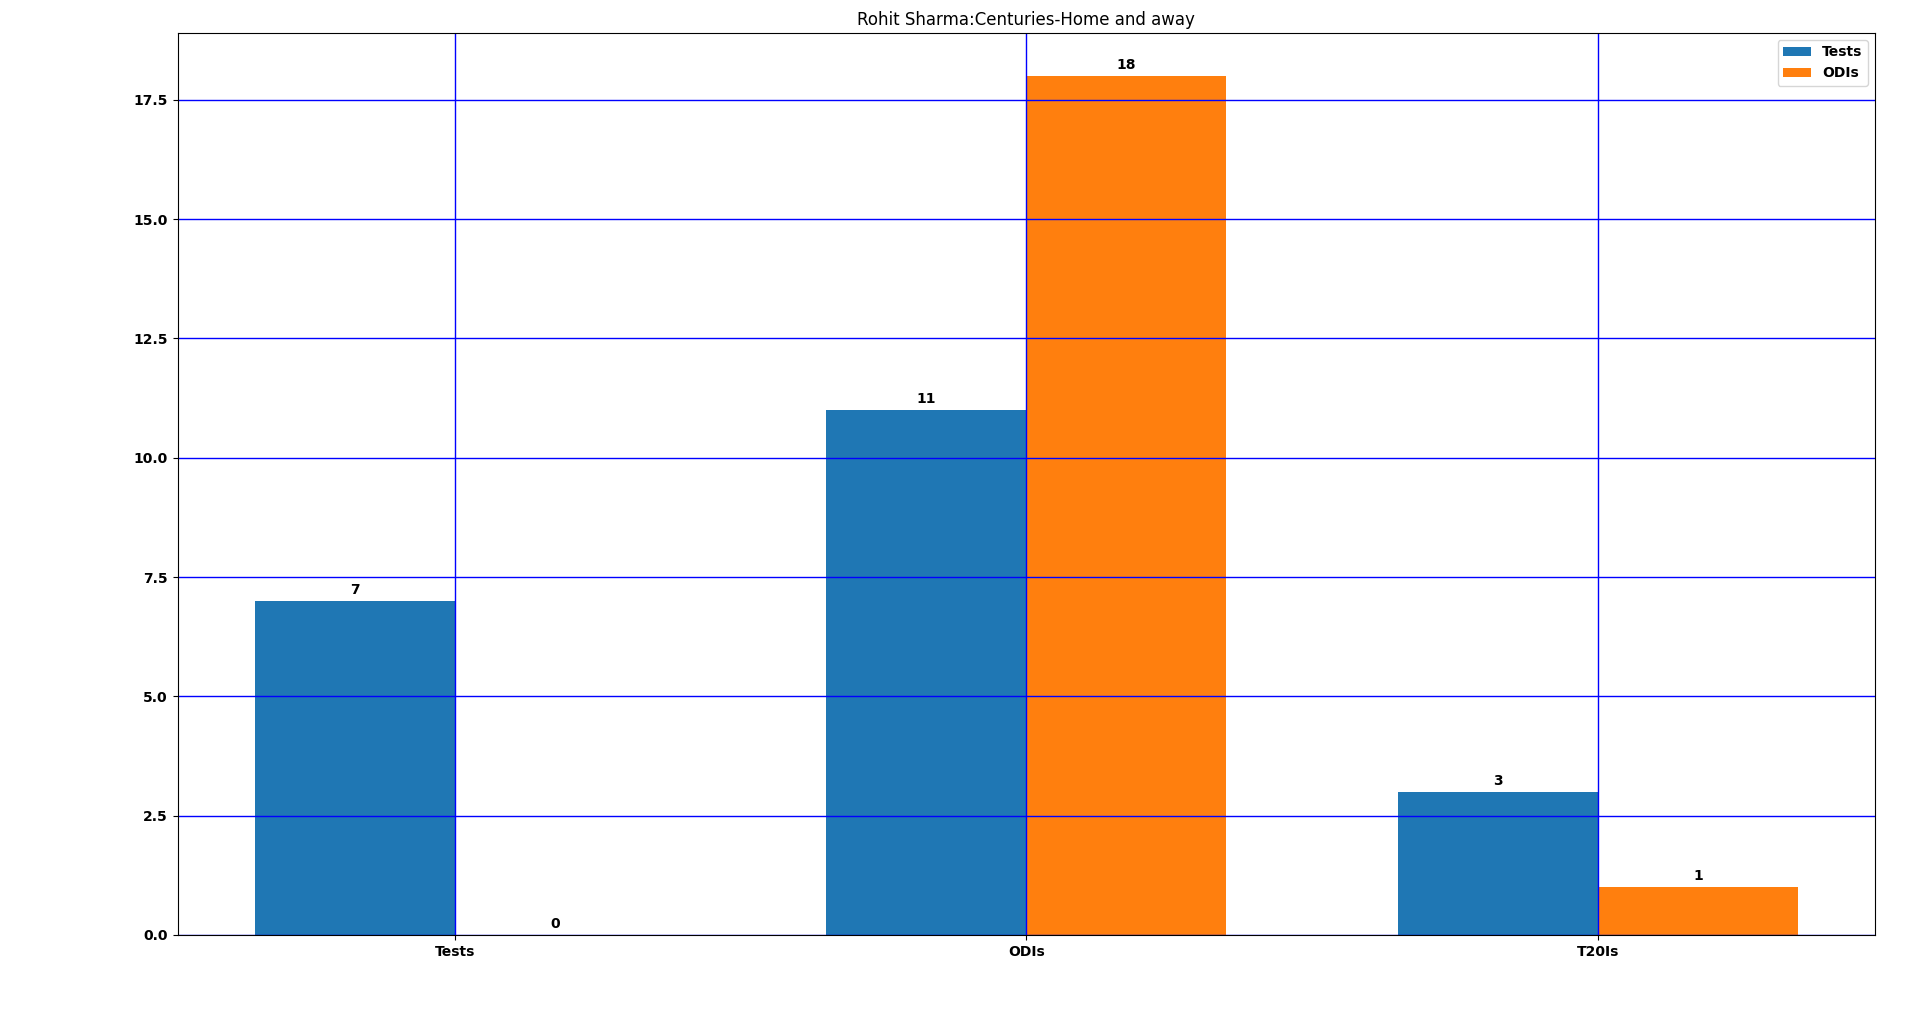
\includegraphics[scale=0.22]{Home_away_centuries.png}
\subsection{Indian Premier League}
When commentators hear the name "Rohit Sharma", they would describe him as someone who has the unbelievable capability of hitting humongous sixes just based on his timing. He is such a sweet timer of the ball, that people associate the term "lazy elegance" with him.
The scatter plot below shows the top 10 all time IPL six hitters, and their strike rate.Featuring in the top 10, is a great deal. Besides, having a 130+ strike rate, and hitting 201 odd sixes, just proves how entertaining Rohit is, and probably explains why people are crazy behind the "hitman". 
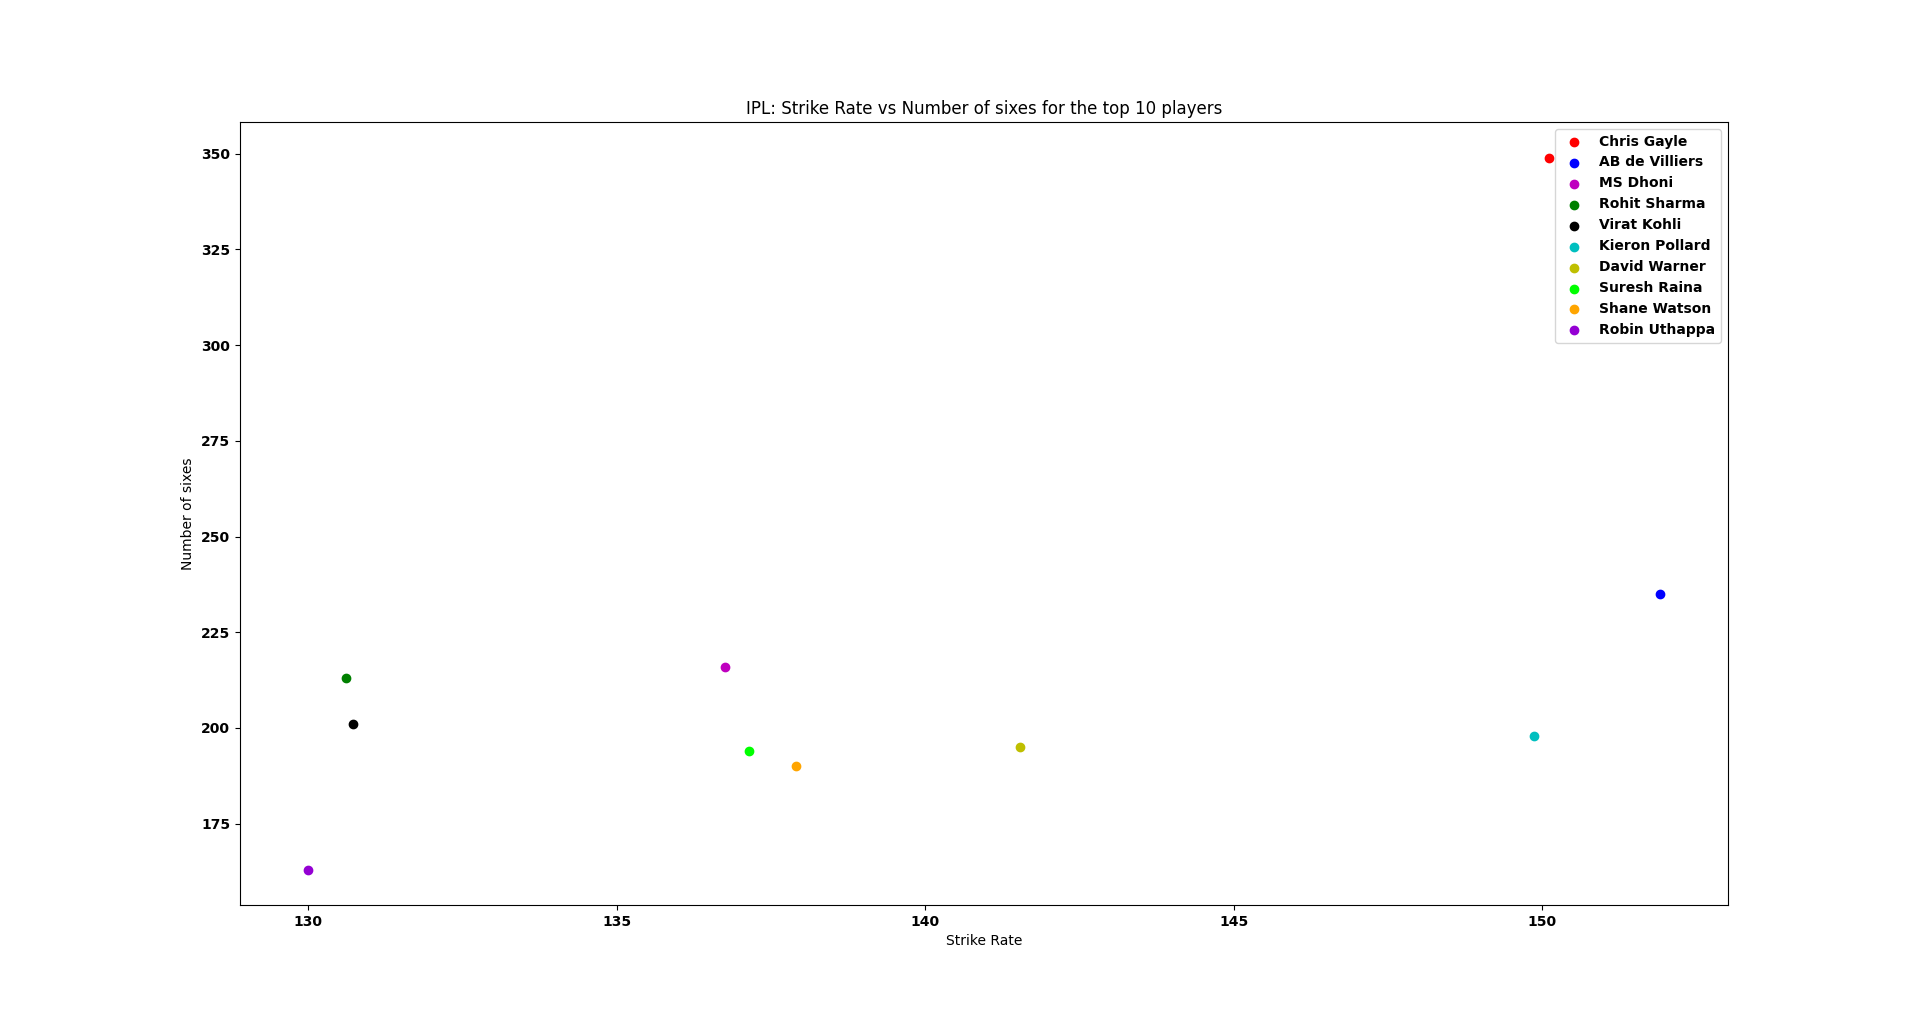
\includegraphics[scale=0.3]{ipl_.png}
\section{Achievements}
1. Arjuna Award\\
2. Rajiv Gandhi Khel Ratna\\
3. ICC ODI Player of the year:2019\\
4. ICC ODI Team of the year: 2014,2016,2017,2018,2019\\
% \newpage
\section{References}
\begin{flushleft}
        1. \href{https://en.wikipedia.org/wiki/Rohit_Sharma}{Wikipedia}\\
        2. \href{https://www.espncricinfo.com/india/content/player/34102.html}{ESPN Cricinfo}\\
        3. \href{http://howstat.com/cricket/Statistics/Players/PlayerOverviewSummary.asp?PlayerID=3474}{Howstat}\\
        4. \href{https://www.iplt20.com/stats/all-time/most-sixes}{IPL Stats}
\end{flushleft}
\end{document}